\documentclass[a4paper,12pt]{article}

\usepackage{url}
\usepackage{epsfig}
\usepackage{graphics}
\usepackage{fancyhdr}

\graphicspath{{pictures/}}

\title{Report template for the project in the course DD2380 at KTH}
\author{\hspace*{-0.5cm}
GROUP31\\
\begin{tabular}{cc}
Akash Patel & Christoph Kaiser \\
BIRTHDATE1 & 16/04/92 \\
MAIL1@kth.se & MAIL2@kth.se \\
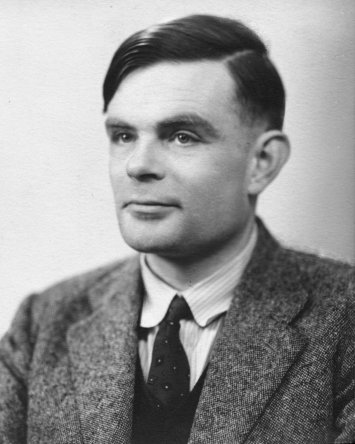
\includegraphics[width=0.13\linewidth]{Alan_Turing_photo} & 
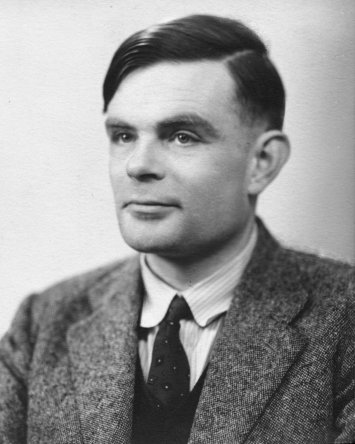
\includegraphics[width=0.13\linewidth]{Alan_Turing_photo} \\
& \\
 Lisa Schmitz & Nikolaos Tatarakis\\
 19920606-T203		&\\
 06/06/92 & BIRTHDATE4 \\
 lschmitz@kth.se & MAIL4@kth.se \\

\includegraphics[width=0.13\linewidth]{lisaSchmitz_photo} &
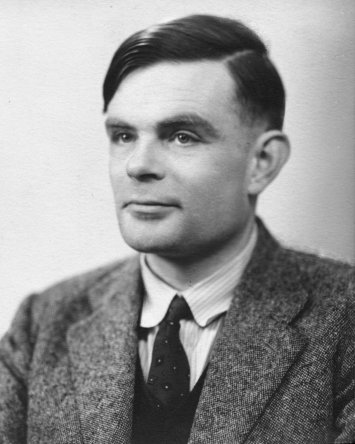
\includegraphics[width=0.13\linewidth]{Alan_Turing_photo}
\end{tabular}} 
% Normally there will not be any pictures but we want
% these so that we can connect faces to names in the course
% We also want birthdates so that we can tell people with the same
% name apart
\date{}

\pagestyle{fancy}
\setlength{\headheight}{15pt}
\fancyhf{}
\lhead{DD2380 ai15} % DO NOT REMOVE!!!!
\rhead{A. Patel, C. Kaiser, L. Schmitz, N. Tatarakis} %% UPDATE WITH YOUR NAMES

\begin{document}

\maketitle
\thispagestyle{fancy}

\begin{abstract}

\end{abstract}
This paper explores the potential accuary of the analysis of song lyrics. Different text analysers were tested for their ability to categorize lyrics as \textit{negative} or \textit{positive}. The focus lies on the comparison of different feature extraction methods and classifier. The identification of emotion in lyrics is a problem which has no satisfying solution yet.

\clearpage

%%%%%%%%%%%%%%%%%%%%%%%%%%%%%%%%%%%%%%%%%%%%%%%%%%%%%%%%%%%%%
%%%%%%%%%%%%%%%%%%%%%%%%%%%%%%%%%%%%%%%%%%%%%%%%%%%%%%%%%%%%%
\section*{NOTE}
Related Works, Experimental Results, Discussions, Summary are sections that MUST be contained.

 The section \textit{Contributions} is a place to express any difference in contributions. The default assumption is that you all agree that all of you had an equal part to play in the project.

\section{Introduction (1--2 pages)}
\label{sec:intro}

Music has a great impact on people. Everyone knows the phenomen that a song can influence our mood, it can make us sad and it can make us happy. This amazing control over people's feelings is something which can be used for many different purposes. For example music provider like Spotify offer playlists labelled with a certain mood. But industries are not the only area of application. Researchers see a use for it in edutainment and even psychological therapy. Unfortunately, the task of predicting the correct assoziated mood is not an easy one due to the comlexity of how emotion is transferred in songs. Obviously emotion is encoded both in the audio and the lyrics of a song\,\cite{yang2008regression}. This paper compares methods to identify emotion by analysing the text of song lyrics. In order to avoid unnecessary difficulties for the comparision we decided to use only two categories by dividing the songs into some with a positive and others with a negative mood. As the results of other research studies suggest, this is even not easy to accomplish in a sufficient way.

\subsection{Contribution}
Bla bla bla bla bla bla bla bla bla bla bla bla bla bla bla bla bla 
bla bla bla bla bla bla bla bla bla bla bla bla bla bla bla bla bla 
bla bla bla bla bla bla bla bla bla bla bla bla bla bla bla bla bla 
bla bla bla bla bla bla bla bla bla bla bla bla bla bla bla bla bla

\subsection{Outline}
Bla bla bla bla bla bla bla Section~\ref{sec:relwork} bla bla bla bla 
bla bla bla bla bla Section~\ref{sec:method} bla bla bla bla bla bla 
bla bla bla bla bla bla bla bla bla bla bla Section~\ref{sec:exps}
bla bla bla bla bla bla Section~\ref{sec:summary} bla bla bla bla bla

%%%%%%%%%%%%%%%%%%%%%%%%%%%%%%%%%%%%%%%%%%%%%%%%%%%%%%%%%%%%%
%%%%%%%%%%%%%%%%%%%%%%%%%%%%%%%%%%%%%%%%%%%%%%%%%%%%%%%%%%%%%
\section{Related work}
\label{sec:relwork}

Bla bla bla bla bla bla bla bla bla bla bla bla bla bla bla bla bla 
bla bla bla bla bla bla bla bla bla bla bla bla bla bla bla bla bla 
bla bla bla bla bla bla bla bla bla bla bla bla bla bla bla bla bla 
bla bla bla bla bla bla bla bla bla bla \cite{RussellNorvigAIBook3rd}
bla bla bla bla bla bla

%%%%%%%%%%%%%%%%%%%%%%%%%%%%%%%%%%%%%%%%%%%%%%%%%%%%%%%%%%%%%
%%%%%%%%%%%%%%%%%%%%%%%%%%%%%%%%%%%%%%%%%%%%%%%%%%%%%%%%%%%%%
\section{My method}
\label{sec:method}

Bla bla bla bla bla bla bla bla bla bla bla bla bla bla bla bla bla 
bla bla bla bla bla bla bla bla bla bla bla bla bla bla bla bla bla 
bla bla bla bla bla bla bla bla bla bla bla bla bla bla bla bla bla 

\subsection{Implementation}
\label{sec:impl}

Bla bla bla bla bla bla bla bla bla bla bla bla bla bla bla bla bla 
bla bla bla bla bla bla bla bla bla bla bla bla bla bla bla bla bla 
bla bla bla bla bla bla bla bla bla bla bla bla bla bla bla bla bla 

%%%%%%%%%%%%%%%%%%%%%%%%%%%%%%%%%%%%%%%%%%%%%%%%%%%%%%%%%%%%%
%%%%%%%%%%%%%%%%%%%%%%%%%%%%%%%%%%%%%%%%%%%%%%%%%%%%%%%%%%%%%
\section{Experimental results}
\label{sec:exps}

Bla bla bla bla bla bla bla bla bla bla bla bla bla bla bla bla bla 
bla bla bla bla bla bla bla bla bla bla bla bla bla bla bla bla bla 
bla bla bla bla bla bla bla bla bla bla bla bla bla bla bla bla bla 

\subsection{Experiemntal setup}
Bla bla bla bla bla bla bla bla bla bla bla bla bla bla bla bla bla 
bla bla bla bla bla bla bla bla bla bla bla bla bla bla bla bla bla 
bla bla bla bla bla bla bla bla bla bla bla bla bla bla bla bla bla 

\subsection{Experiment ...}

Bla bla bla bla bla bla bla bla bla bla bla bla bla bla bla bla bla 
bla bla bla bla bla bla bla bla bla bla bla bla bla bla bla bla bla 
bla bla bla bla bla bla bla bla bla bla bla bla bla bla bla bla bla 

\begin{figure}
\centering
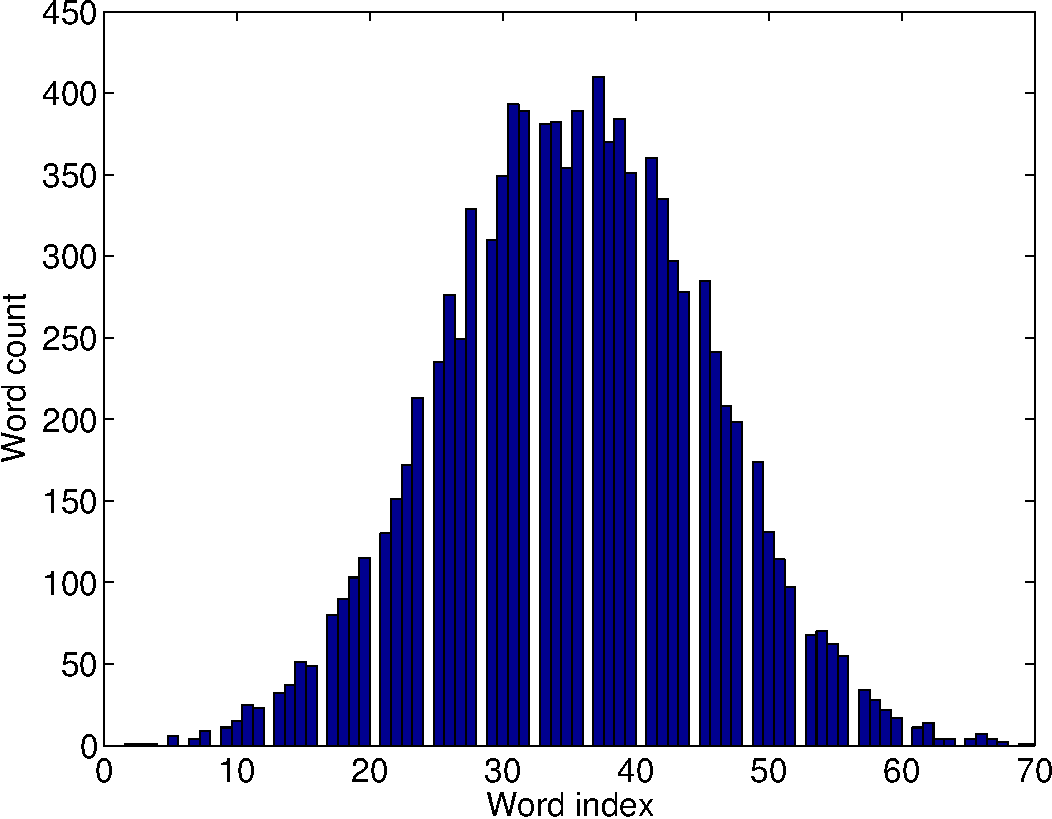
\includegraphics[width=0.8\linewidth]{histogram}
\caption{A description that makes browsing the paper easy and clearly 
describes what is in the picture. Make sure that the text in the figure 
is large enough to read and that the axes are labelled.}
\label{fig:histogram}
\end{figure}

Bla bla bla bla bla Figure~\ref{fig:histogram} bla bla bla bla bla bla 
bla bla bla bla bla bla bla bla bla bla bla bla bla bla bla bla bla 
bla bla bla bla bla bla bla bla bla bla bla bla bla bla bla bla bla 

\begin{table}
\begin{center}
\begin{tabular}{|c|c|c|}
\hline
Bla bla & Bla bla & Bla bla \\ \hline
42 & 42 & 42 \\ \hline
42 & 42 & 42 \\ \hline
\end{tabular}
\caption{A description that makes browsing the paper easy and clearly 
describes what is in the table.}
\label{tab:results}
\end{center}
\end{table}

Bla bla bla bla bla Table~\ref{tab:results} bla bla bla bla bla bla 
bla bla bla bla bla bla bla bla bla bla bla bla bla bla bla bla bla 
bla bla bla bla bla bla bla bla bla bla bla bla bla bla bla bla bla 

%%%%%%%%%%%%%%%%%%%%%%%%%%%%%%%%%%%%%%%%%%%%%%%%%%%%%%%%%%%%%
%%%%%%%%%%%%%%%%%%%%%%%%%%%%%%%%%%%%%%%%%%%%%%%%%%%%%%%%%%%%%
\section{Summary and Conclusions}
\label{sec:summary}

Bla bla bla bla bla bla bla bla bla bla bla bla bla bla bla bla bla 
bla bla bla bla bla bla bla bla bla bla bla bla bla bla bla bla bla 
bla bla bla bla bla bla bla bla bla bla bla bla bla bla bla bla bla 


%%%%%%%%%%%%%%%%%%%%%%%%%%%%%%%%%%%%%%%%%%%%%%%%%%%%%%%%%%%%%
%%%%%%%%%%%%%%%%%%%%%%%%%%%%%%%%%%%%%%%%%%%%%%%%%%%%%%%%%%%%%
\section{Contributions}
\label{sec:contributions}
We the members of project groupXX unanimously declare that 
we have all equally contributed toward the completion of this
project. (PLEASE CHANGE THIS SUITABLY WITH DETAILS, IF IT IS NOT TRUE)


%%%%%%%%%%%%%%%%%%%%%%%%%%%%%%%%%%%%%%%%%%%%%%%%%%%%%%%%%%%%%
%%%%%%%%%%%%%%%%%%%%%%%%%%%%%%%%%%%%%%%%%%%%%%%%%%%%%%%%%%%%%
\bibliographystyle{plain}
\bibliography{reflist}


\end{document}